\documentclass[10pt,a4paper]{article}
\usepackage[singlespacing, onehalfspacing]{setspace}
\usepackage{parskip}
\usepackage[spaces,hyphens]{url}
\usepackage{enumitem}
\usepackage[left=3cm,right=3cm,top=3cm,bottom=3cm]{geometry}
\usepackage{titlesec}
\usepackage{fancyhdr}
\usepackage{tocloft}
\usepackage{longtable}
\usepackage{tabularx}
\usepackage{booktabs}
\usepackage{caption}
\usepackage{amsmath}
\usepackage{amssymb}
\usepackage{colortbl}
\usepackage{tikz}
\usepackage{pgfplots}
\usepackage{pdflscape}
\usepackage{pbox}
\usepackage{dcolumn}
\usepackage[figuresleft]{rotating}
\usepackage{subcaption}
\usepackage{tcolorbox}
\usepackage{listings}
\usepackage[export]{adjustbox}

\usepackage[backend=biber, style=authoryear-comp, sorting=nyt, url=false, isbn=false, doi=false, clearlang=false, maxbibnames=10, maxcitenames=2]{biblatex}
\addbibresource{../library.bib}

\pgfplotsset{compat=1.17}

\usepackage[colorlinks = true,
            linkcolor = PN1,
            urlcolor  = F3,
            citecolor = F3,
            anchorcolor = A4]{hyperref}

% - Polar Night
\definecolor{PN0}{RGB}{64,52,64}
\definecolor{PN1}{RGB}{59,66,82}
\definecolor{PN2}{RGB}{67,76,94}
\definecolor{PN3}{RGB}{76,86,106}

% - Snow Storm
\definecolor{SS0}{RGB}{216,222,233}
\definecolor{SS1}{RGB}{229,233,240}
\definecolor{SS2}{RGB}{236,239,244}

% - Frost
\definecolor{F0}{RGB}{143,188,187}
\definecolor{F1}{RGB}{136,192,208}
\definecolor{F2}{RGB}{129,161,193}
\definecolor{F3}{RGB}{94,129,172}

% - Aurora
\definecolor{A0}{RGB}{191,97,106}
\definecolor{A1}{RGB}{208,135,112}
\definecolor{A2}{RGB}{235,203,139}
\definecolor{A3}{RGB}{163,190,140}
\definecolor{A4}{RGB}{180,142,173}

\definecolor{light-gray}{gray}{0.95}

\newcommand{\tabitem}{~~\llap{\textbullet}~~}
\newcommand{\oarrow}{\textcolor{A1}{$\rightarrow$} }
\newcommand{\rarrow}{\textcolor{A0}{$\rightarrow$} }
\newcommand{\garrow}{\textcolor{F1}{$\rightarrow$} }

\lstset{language=R,
    basicstyle=\fontsize{8}{9}\selectfont\ttfamily,
    backgroundcolor = \color{light-gray},
    %stringstyle=\color{F3},
    %otherkeywords={0,1,2,3,4,5,6,7,8,9},
    %morekeywords={TRUE,FALSE},
    deletekeywords={data,frame,length,as,character},
    %keywordstyle=\color{A1},
    commentstyle=\color{PN3},
    showstringspaces=false,
    rulecolor=\color{black},
    frameshape={RYR}{Y}{Y}{RYR}
}

\widowpenalty90000
\clubpenalty90000

\pagestyle{fancy}
\setlength{\headheight}{15pt}
\fancyhf{}
\fancyhead[R]{\thepage}
\fancyhead[L]{\textit{Data Science 101 -- Regressionen}}
\titleformat*{\section}{\large\bfseries}
\renewcommand\cftsecfont{\normalsize}
\renewcommand\cftsecpagefont{\footnotesize\bfseries}
\renewcommand{\cftsecleader}{\cftdotfill{\cftdotsep}}
\setlength{\cftbeforesecskip}{-2pt}
\renewcommand{\abstractname}{}

\makeatletter
\setlength{\@fptop}{0pt}
\setlength{\parskip}{0.5pt}
\makeatother

\renewcommand{\contentsname}{Übersicht}

\begin{document}

\thispagestyle{empty}
\frenchspacing
\begin{flushleft}
\begin{tabular}{p{11.5cm} r}
Martin Kerntopf & 25. Januar 2022 \\
Email: martin.kerntopf@uni-greifswald.de \\
Seminar: Data Science für Geistes- und Sozialwissenschaftler 
\end{tabular}
\end{flushleft}
\hrule
\begin{center}
\vspace{0.4cm}
\large{\textsc{Regressionsanalyse}}

V 0.1

\vspace{0.4cm}
\end{center}
%\vspace{-0.2cm}
\hrule 
%\vspace{0.2cm}
\frenchspacing

\tableofcontents

\section{Einleitung}
In diesem Script finden Sie eine Zusammenfassung und weiterführende Erläuterung der im Seminar benutzten begriffe und Verfahren. Zentral hierbei ist die Auflistung der wichtigsten Begrifflichkeiten und Konzepte im Zusammenhang mit dem Thema der Regressionsanalysen. Dies wird ergänzt durch eine Kurzbeschreibung der zentralen Annahmen im Zusammenhang mit der Durchführung einer Regressionsanalyse. Folgend werden zentrale Begriff im Bereich der Ergebnisauswertung und -überprüfung aufgeführt. %Anhand einiger Praxisbeispiele werden die genannten Verfahren und Begriffe zusätzlich veranschaulicht.
    \subsection{Werte}
        \subsection{Koeffizienten}
            \begin{itemize}
                \item a = Der Schnittpunkt mit  der y-Achse, wenn x = 0 ist
                \item b = Die Steigung der Geraden, wenn x um 1 erhöht wird
            \end{itemize}

            \subsection{Fehlerterm}
            \begin{itemize}
                \item $\epsilon$ = unbeobachtbare Zufallsvariablen, die den vertikalen Abstand zwischen Beobachtungspunkt und wahrer Gerade messen. Für sie nimmt man für gewöhnlich an, dass sie unkorreliert sind, einen Erwartungswert von Null und eine homogene Varianz aufweisen. Sie beinhalten unbeobachtete Faktoren, die sich auf die abhängige Variable auswirken.
            \end{itemize}

        \subsection{Residuen}
            \begin{itemize}
                \item Residuen messen den vertikalen Abstand zwischen Beobachtungspunkt und der geschätzten Regressionsgerade. Diese Abstände sind für die Ermittlung der kleinsten Quadrate (Ordinary Least Squares -- OLS) relevant
            \end{itemize}
    \subsection{Grundannahmen}
        \subsubsection{Der Erwartungswert der Residuen ist Null}
        Die erste Annahme geht davon aus, dass die Fehlerterme im Durchschnitt Null ergeben (genannt Erwartungswert). Es gibt sowohl Abweichungen gegen unten als auch gegen oben. Im Schnitt heben sich diese jedoch auf. Deshalb werden auch die Quadratterme der Residuen minimiert und nicht die Residuen selber, da bei Quadratwerten sich negative und positive Abweichungen nicht aufheben.

        \subsubsection{Fehlerterme sind unkorreliert}
        Die zweite Annahme ist eine sehr wichtige Annahme. Sie besagt, dass die Residuen nicht miteinander korrelieren. Dies tun sie dann, wenn wichtige Variablen nicht in das Modell aufgenommen wurden.

        \subsubsection{Homo- und Heteroskedastizität}
        Die Homoskedastizität besagt, dass die Varianz der Fehlerterme gleichmässig verteilt ist. Ist dies nicht der Fall spricht man von Heteroskedastizität. Liegt Heteroskedastizität vor, ist OLS nicht mehr effizient und es müssen andere Verfahren angewandt werden. Kann optisch oder via Breush Pagan Test ermittelt werden (bei signifikante p-Wert im BPT liegt Heteroskedastizität vor).

        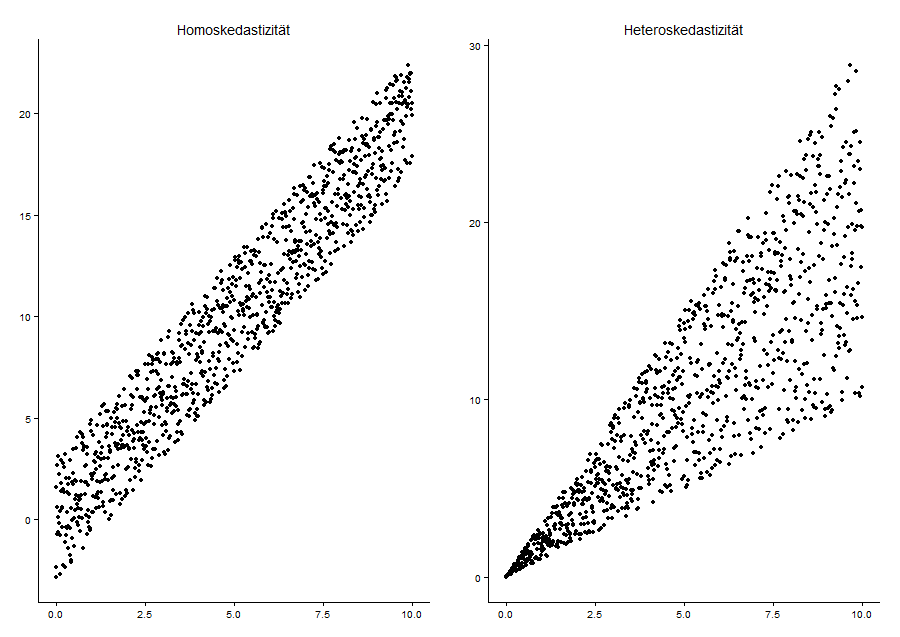
\includegraphics[max width=\textwidth]{../Plots/homo_heterosked.png}

        \subsubsection{Fehlerterme sind normalverteilt}
        Die Normalverteilung (auch Gauss-Verteilung genannt) ist eine stetige Verteilung. Viele Fehler lassen sich durch diese symmetrische Verteilung erklären.


\section{Ergebnis auswerten und überprüfen}
    \subsection{p-Wert -- Statistische Signifikanz}
    Wird ein statistisches Ergebnis als signifikant bezeichnet, so drückt dies aus, dass die Irrtumswahrscheinlichkeit, eine angenommene Hypothese treffe auch auf die Grundgesamtheit zu, nicht über einem festgelegten Niveau liegt. Anders ausgedrückt: in gemessener Zusammenhang zwischen zwei Variablen tritt in der Stichprobe nicht einfach zufällig auf, sondern trifft auch für die Grundgesamtheit zu. Auf Signifikanz geprüft werden können nur Hypothesen, nicht das Ergebnis von Einzelmerkmalen. 

    \begin{itemize}
        \item Der p-Wert bewegt sich zwischen 0 und 1, je kleiner er ist, desto signifikanter das Ergebnis
        \item p $\leq $ 0.05 bedeutet das die Nullhypothese zurückgewiesen wird
        \item p $ > $ 0.05 heißt das die Alternativhypothese nicht anzunehmen ist. Damit wird die Nullhypothese angenommen 
    \end{itemize}

    \subsection{R\textsuperscript{2} -- Goodness of Fit}
    Nach dem eine Regression durchgeführt wurde bleibt meist noch die Frage, wie gut das Regressionsmodell denn die Daten nun tatsächlich erklären kann, d.h. wie gut die Regressionsgerade zu den
    Daten ``passt.'' Um diese Frage zu beantworten wird der Coefficient of Determination verwendet,
    der auch als R-squared bzw. R\textsuperscript{2}-Wert bezeichnet wird. Der R\textsuperscript{2}-Wert ermittelt, welcher Anteil der Gesamtvarianz in den Daten durch die Regressionsgerade erklärt werden kann.

    \begin{itemize}
        \item R\textsuperscript{2} repräsentiert den Anteil an der Gesamtvariabilität in y an, der mit dem Regressionsmodell mittels der unabhängigen Variable x erklärt werden kann
        \item R\textsuperscript{2} ist ein Wert zwischen 0 und 1, je näher der R\textsuperscript{2}-Wert an 1 ist, desto besser passt die Regressionsgerade zu den Daten
        \item Ein R\textsuperscript{2}-Wert von z.B. 0.24 bedeutet, dass 24\% der Variabilität der abhängigen Variable y mit dem Regressionmodell durch die unabhängige Variable x erklärt werden kann
        \item Der Adjusted R\textsuperscript{2}-Wert wird genutzt wenn das Modell mehrere unabhängige Variablen aufweist, da der Multiple R\textsuperscript{2}-Wert mit zunehmender Anzahl unabhängiger Variablen automatisch steigt
    \end{itemize}

    \subsection{Multikolliniarität}
    \begin{itemize}
        \item Liegt dann vor, wenn mehrere unabhängige Variablen in einer Regressionsanalyse (stark) miteinander korrelieren
        \item[] \oarrow Variance Inflation Factor (VIF) Test
        \begin{itemize}
            \item[] \begin{lstlisting}
install.packages('regclass') # Das Package das den Test bereitstellt
VIF(modell_name)
            \end{lstlisting}
        \item Generell wird bei einem Ergebniswert von 5 bis 10 angenommen, das Multikolliniarität vorliegt
        \end{itemize}
    \end{itemize}

    \subsection{Heteroskedastizität}
        \begin{itemize}
            \item 
            Breush Pagan Test
        \end{itemize}


%\section{Praxis}


\section{Weiterführende Literatur}
\begin{itemize}
    \item \fullcite{Hedderich2016} 
    \item \fullcite{Wolf2010}
    \item \fullcite{Ciaburro2018}
    \item \fullcite{Pardoe2020}
  \end{itemize}
\end{document}